\documentclass[12pt]{article}

% Paquetes básicos
\usepackage[utf8]{inputenc}
\usepackage[T1]{fontenc}
\usepackage[spanish,shorthands=off]{babel}
\usepackage{amsmath,amssymb,amsthm}
\usepackage{geometry}
\usepackage{fancyhdr}
\usepackage{graphicx}
\usepackage{setspace}
\usepackage{hyperref}
\usepackage{tikz}
\usetikzlibrary{calc}
\usepackage{float}
\usepackage{bigints}
\usepackage{pgfplots}
\pgfplotsset{compat=1.18}

\geometry{margin=2.5cm}

\onehalfspacing

\pagestyle{fancy}
\fancyhf{}

\title{
    \textbf{\Huge{Campos eléctricos}}\\[0.3cm]
    \large{Ezequiel}
}

\date{\today}

\begin{document}

\maketitle

\section{Introducción}
El propósito de este ensayo experimental es mapear el campo eléctrico generado entre dos placas conductoras paralelas utilizando papel semiconductor. A partir de la caracterización de las superficies equipotenciales en el sistema, se busca demostrar experimentalmente la uniformidad del campo eléctrico en la región central del arreglo. Para la recolección de datos se empleó una fuente de alimentación de bajo voltaje ajustada a un rango operacional de $1\text{ V}$ a $8\text{ V}$, un voltímetro digital con puntas de prueba, papel carbón para el trazado de puntos equipotenciales, y un conjunto de conectores con pinzas cocodrilo y prensas de soporte para garantizar un contacto eléctrico estable a lo largo del plano de medición.

\section{Modelo Físico-Matemático}
Un campo eléctrico uniforme se define como una región del espacio donde el vector campo eléctrico $\overrightarrow{E}$ conserva su magnitud, dirección y sentido en todos los puntos. Matemáticamente, la magnitud del campo en una dimensión se relaciona con la variación del potencial eléctrico mediante la expresión $\overrightarrow{E} = -\frac{\Delta V}{\Delta x}$. La intensidad del campo es directamente proporcional a la diferencia de potencial aplicada e inversamente proporcional a la distancia de separación entre los conductores. La orientación vectorial resulta perpendicular a la geometría de las placas; de esta forma, en arreglos con placas horizontales el campo sigue la dirección del eje $\overrightarrow{Oy}$, mientras que en placas verticales se orienta según el eje $\overrightarrow{Ox}$.

El potencial eléctrico $V$ en un punto del espacio representa la energía potencial por unidad de carga necesaria para trasladar una carga de prueba en presencia del campo. Formalmente, la diferencia de potencial entre dos puntos $A$ y $B$ se define como:
\begin{equation}
    \Delta V = -\int_{A}^{B} \overrightarrow{E} \cdot d\overrightarrow{l}
\end{equation}
donde $d\overrightarrow{l}$ representa el vector desplazamiento infinitesimal a lo largo de la trayectoria. Si la fuerza eléctrica conservativa sobre la carga es $\overrightarrow{F} = q\overrightarrow{E}$, el trabajo realizado por el campo al desplazar la carga equivale a $W_{AB} = q \int_{A}^{B} \overrightarrow{E} \cdot d\overrightarrow{l}$. Por consiguiente, la variación de energía potencial es $\Delta U = -W_{AB}$, reafirmando que $\Delta V = \frac{\Delta U}{q} = -\int_{A}^{B} \overrightarrow{E} \cdot d\overrightarrow{l}$.

Para el caso particular de un campo uniforme orientado a lo largo del eje $x$, las componentes ortogonales del campo son nulas ($E_x = E = \text{cte.}$), por lo que la integral de línea se simplifica a una relación lineal directa entre el potencial y la posición: $\Delta V = -E (x_B - x_A)$.

\begin{figure}[H]
    \centering
    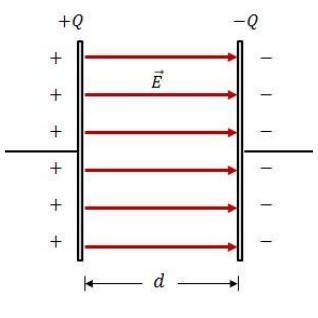
\includegraphics[width=0.5\linewidth]{Demostración de las interacciones entre partículas y líneas de campo.jpg}
    \caption{Demostración de las interacciones entre partículas y líneas de campo.}
    \label{fig:placeholderA}
\end{figure}

Desde el punto de vista del procesamiento analítico, esta relación describe una función lineal de primer grado de la forma $y = mx + b$, donde la pendiente $m = \frac{\Delta y}{\Delta x}$ representa la tasa de cambio instantánea del potencial respecto a la posición. En términos de cálculo diferencial, la derivada de una función constante es nula ($f(x)=c \rightarrow f'(x)=0$), mientras que la derivada de una función de potencia cumple que para $f(x)=ax^n$, $f'(x)=nax^{n-1}$, con su correspondiente operación inversa definida mediante la integral $\int ax^b \, dx = \frac{ax^{b+1}}{b+1}$.

\begin{figure}[H]
    \centering
    \begin{tikzpicture}[scale=1, thick]
        \draw[step=1cm,gray!30,very thin] (-5,-5) grid (5,5);
        \draw[->, thick] (-5,0) -- (5,0) node[right] {$x$};
        \draw[->, thick] (0,-5) -- (0,5) node[above] {$y$};
        \draw[thick] (1,1) -- (2,1);
        \draw[thick] (2,1) -- (2,2);
        \draw[domain=-5:5,smooth,thick,blue] plot (\x,{\x});
        \draw[domain=-3.16:3.16, smooth, thick, red] plot (\x,{pow(\x,2)/2});
    \end{tikzpicture}
    \caption{Representación gráfica del comportamiento funcional $f(x)=\frac{x^2}{2}$ y su derivada $f'(x)=x$.}
    \label{fig:placeholderB}
\end{figure}

\section{Metodología de simulación}
El montaje experimental se estructuró superponiendo secuencialmente una hoja A4 de registro, una lámina de papel carbón, la hoja de mapeo semiconductora y las pinzas de soporte encargadas de fijar el conjunto. La fuente de alimentación se conectó a los extremos de la hoja de papel semiconductor mediante cables con pinzas cocodrilo para fijar las condiciones de contorno electrostáticas.

Para el registro de datos, se aplicó un voltaje inicial $V_0 = 1\text{ V}$ y un voltaje final $V_f = 8\text{ V}$. El procedimiento consistió en marcar iterativamente 5 puntos equipotenciales por cada incremento discreto de $1\text{ V}$, obteniendo un total de 40 muestras experimentales. Posteriormente, se retiró la hoja A4 y se promediaron las lecturas para cada valor de potencial trazando líneas rectas representativas. Finalmente, se midió la distancia relativa $\Delta x$ desde la primera línea de referencia ($1\text{ V}$) hacia cada una de las equipotenciales subsiguientes, tabulando los pares ordenados de voltaje en función de la posición.

\section{Análisis de resultados}
Los pares ordenados obtenidos experimentalmente de potencial $V$ y distancia relativa $\Delta x$ se presentan en la Figura \ref{fig:placeholder}. La regresión lineal aplicada a los datos experimentales arrojó la ecuación de ajuste $y = 34.646x + 1$, la cual responde de manera precisa al modelo teórico $y = mx + b$. La derivada de esta función ajustada representa la magnitud del campo eléctrico $y' = 34.646\text{ V/m} = |\overrightarrow{E}|$.

\begin{figure}[H]
    \centering
    \begin{minipage}{0.4\textwidth}
        \centering
        \begin{tabular}{|c|c|}
        \hline
        $V$ (V) & $\Delta x$ (m) \\ \hline
        1  & 0.000 \\ 
        2  & 0.031 \\ 
        3  & 0.060 \\ 
        4  & 0.086 \\ 
        5  & 0.116 \\ 
        6  & 0.146 \\ 
        7  & 0.174 \\ 
        8  & 0.203 \\ 
        \hline
        \end{tabular}
    \end{minipage}%
    \hfill
    \begin{minipage}{0.55\textwidth}
        \centering
        \begin{tikzpicture}
          \begin{axis}[
            axis lines=middle,
            grid=both,
            xmin=0, xmax=0.2,
            ymin=0, ymax=10,
            xlabel={$\Delta x$}, xlabel style={at={(axis description cs:1.05,0)}, above}, ylabel={$V$}, ylabel style={at={(axis description cs:0,1.05)}, right},
            samples=200,
            domain=0:0.2,
            xtick={0,0.05,0.1,0.15,0.2},
            scaled ticks=false,
            xticklabel style={/pgf/number format/fixed},
            width=10cm, height=10cm
          ]
            \addplot[red, thick] {34.646*x + 1};
            \addplot[only marks, mark=*] coordinates {(0,1) (0.031,2) (0.06,3) (0.086,4) (0.116,5) (0.146,6) (0.174,7) (0.203,8)};
          \end{axis}
        \end{tikzpicture}
    \end{minipage}
    \caption{Ajuste lineal del potencial eléctrico en función de la posición.}
    \label{fig:placeholder}
\end{figure}

Para fundamentar analíticamente la constancia de $E$, se deduce formalmente la relación de la diferencia de potencial a partir de los principios del trabajo y la energía. La fuerza eléctrica ejercida sobre una carga $q$ viene dada por:
\begin{equation}
    \overrightarrow{F} = q\overrightarrow{E}
\end{equation}
El trabajo $W_{AB}$ realizado por el campo sobre la carga al desplazarse desde un punto $A$ hasta un punto $B$ se expresa como:
\begin{equation}
    W_{AB} = \int_{A}^{B} \overrightarrow{F} \cdot d\overrightarrow{l} = q \int_{A}^{B} \overrightarrow{E} \cdot d\overrightarrow{l}
\end{equation}
Por definición, la variación de energía potencial eléctrica $\Delta U$ equivale al negativo del trabajo realizado por las fuerzas conservativas del campo:
\begin{equation}
    \Delta U = U(B) - U(A) = -W_{AB}
\end{equation}
Considerando que el potencial eléctrico $V$ representa la energía potencial por unidad de carga ($V = \frac{U}{q}$), la diferencia de potencial resulta:
\begin{equation}
    \Delta V = \frac{\Delta U}{q} = \frac{-W_{AB}}{q}
\end{equation}
Sustituyendo la expresión del trabajo y simplificando la carga de prueba $q$:
\begin{equation}
    \Delta V = -\frac{1}{q} \left( q \int_{A}^{B} \overrightarrow{E} \cdot d\overrightarrow{l} \right) = -\int_{A}^{B} \overrightarrow{E} \cdot d\overrightarrow{l}
\end{equation}
Al restringir el movimiento unidireccional a lo largo del eje $x$, acorde al montaje experimental, la integral adopta la forma:
\begin{equation}
    \Delta V = -\int_{x_A}^{x_B} E_x \, dx
\end{equation}
Dado que el campo eléctrico es uniforme entre las placas paralelas, la componente $E(x) = E$ se mantiene constante y puede extraerse de la integral:
\begin{equation}
    \Delta V = -E \int_{x_A}^{x_B} dx = -E(x_B - x_A)
\end{equation}

Para evaluar la consistencia del modelo, se calculó la diferencia de potencial entre las equipotenciales de $4\text{ V}$ ($x_B = 0.086\text{ m}$) y $2\text{ V}$ ($x_A = 0.031\text{ m}$). Aplicando la relación teórica para un campo uniforme con $E = 34.646\text{ V/m}$:
\begin{equation}
    \Delta V = -E(x_B - x_A) = -34.646 \cdot (0.086 - 0.031) = -1.9055\text{ V} \approx -1.9\text{ V}
\end{equation}

Comparando esta caída de potencial calculada ($-1.9\text{ V}$) con la variación medida directamente en el experimento ($\Delta V = -2.0\text{ V}$), se determina el campo eléctrico nominal requerido $E_{\text{teor}} = \frac{2\text{ V}}{0.055\text{ m}} = 36.3636\text{ V/m}$. Esto resulta en un error relativo del $4.7\%$:
\begin{equation}
    E_{\%} = \frac{|36.3636 - 34.646|}{34.646} \cdot 100 = 4.7\%
\end{equation}

Esta discrepancia del $4.7\%$ deriva de múltiples fuentes de incertidumbre experimental. Por un lado, la medición geométrica de las posiciones $x_A$ y $x_B$ presenta una incertidumbre instrumental de $\pm 1\text{ mm}$, lo que representa una incertidumbre relativa del $1.8\%$ sobre el intervalo $\Delta x = 0.055\text{ m}$. Por otro lado, la suposición de placas infinitas no se cumple estrictamente; las dimensiones finitas del papel semiconductor generan efectos de borde donde las líneas de campo divergen, alterando la uniformidad si las lecturas no se realizan exclusivamente en el centro geométrico del sistema. Asimismo, existen limitaciones inherentes al método indirecto ($\frac{\Delta V}{\Delta x}$) en comparación con medidas directas de campo, además de tolerancias instrumentales del voltímetro ($\pm 0.5\%$), resistencia de contacto en las pinzas y variaciones de conductividad local en el papel semiconductor.

\section{Conclusión}
Los datos experimentales confirman satisfactoriamente la presencia de un campo eléctrico uniforme en la región central entre las placas paralelas. La dependencia del potencial eléctrico con la posición exhibe una linealidad marcada, decreciendo de forma continua desde la placa con mayor potencial hacia la placa negativa. La concordancia entre la magnitud del campo derivada de la pendiente ($34.646\text{ V/m}$) y las caídas de potencial locales —registrando un error relativo acotado al $4.7\%$— valida las hipótesis físicas adoptadas y demuestra el carácter conservativo del campo electrostático en el arreglo probado.

\end{document}